\documentclass[hyperref={unicode=true}, 12pt]{beamer}

\usepackage[T2A]{fontenc}

\usepackage{fontspec}

\usetheme{Copenhagen}



\usepackage{fontspec}
\setmainfont{Noto Serif}
\setsansfont{Noto Sans}
\setmonofont{Noto Sans Mono}

\usepackage{indentfirst}
\usepackage{enumitem}


\setlist{nosep}
\setlist[enumerate]{wide=\parindent, label=\arabic*)}
\setlist[itemize]{wide=\parindent, label=--}

\usepackage{ragged2e}

\setbeamersize{text margin left=0.4cm, text margin right=0.4cm}


\graphicspath{ {./images/} }

\begin{document}
	
	\begin{frame}[t]
		\vspace{3cm}
		\begin{center}
			\fontsize{14}{16}
			\selectfont
			Система фаззинга программного обеспечения на основе эволюционного подхода
		\end{center}
		\vspace{1cm}
		
		\hfill \begin{minipage}{0.35\textwidth}
			\fontsize{8}{10}
			\selectfont
			
			\raggedleft
			
			
			Выполнил \\
			Редькин В.С.
			
			\vspace{0.1cm}
			
			Руководитель \\
			ст. преп. \\
			Долгов Д.А.
		\end{minipage}
	\end{frame}

	\fontsize{12}{15}
	\selectfont
	
	% титульник: тема, я, научрук
	
	% цель и задачи (список)
	
	% атуальность
	
	\begin{frame}[c]{Цель и задачи}
		
		Цель работы -- разработать систему фаззинга програмного обеспечения, использующую основные подходы генетических алгоритмов.
		
		\vspace{0.2cm}
		
		Задачи работы:
		
		\begin{itemize}
				\item разработать систему трассировки
				\item разработать механизм мутации
				\item протестировать систему на уязвимых образцах
		\end{itemize}
		
	\end{frame}

	\begin{frame}{Актуальность}
		\begin{minipage}{0.53\textwidth}
			\raggedright
			\begin{itemize}
				
				\fontsize{12}{15}
				
				\item небезопасные по памяти языки
				
				\item программистам сложно удержать всё в голове
				
				\item кибератаки становятся масштабнее и дороже
			\end{itemize}
		
		\end{minipage}\begin{minipage}{0.47\textwidth}
			\centering
			TIOBE 2023 index
			
			\vspace{0.1cm}
			\begin{tabular}{|c|c|c|}
				\hline
				rank & language & percent \\
				\hline
				1 & Python & 14.83\% \\
				\hline
				2 & C & 14.73\% \\
				\hline
				3 & Java & 13.56\% \\
				\hline
				4 & C++ & 13.29\% \\
				\hline
				5 & C\# & 7.17\% \\
				\hline
			\end{tabular}
		\end{minipage}
		
	\end{frame}

	\begin{frame}[t]{Использованные технологии}
			\vspace{1cm}
		\begin{itemize}
			\fontsize{14}{18}
			\selectfont
			\item КС грамматики для описания ввода
			\item генетические алгоритмы для генерации новых образцов
			\item ptrace для трассировки программы
			\item алгоритмы одноруких бандитов для выбора мутаторов
			\item язык Rust для реализации
		\end{itemize}
		
	\end{frame}

	% а дальше уже по работе

	\begin{frame}{Фаззинг}
		\begin{minipage}{0.6\textwidth}
			
			\begin{itemize}
				\item мутируем данные
				
				\item подаём на вход программе
				
				\item ищем segfault
			\end{itemize}
			
		\end{minipage}\begin{minipage}{0.43\textwidth}
		
		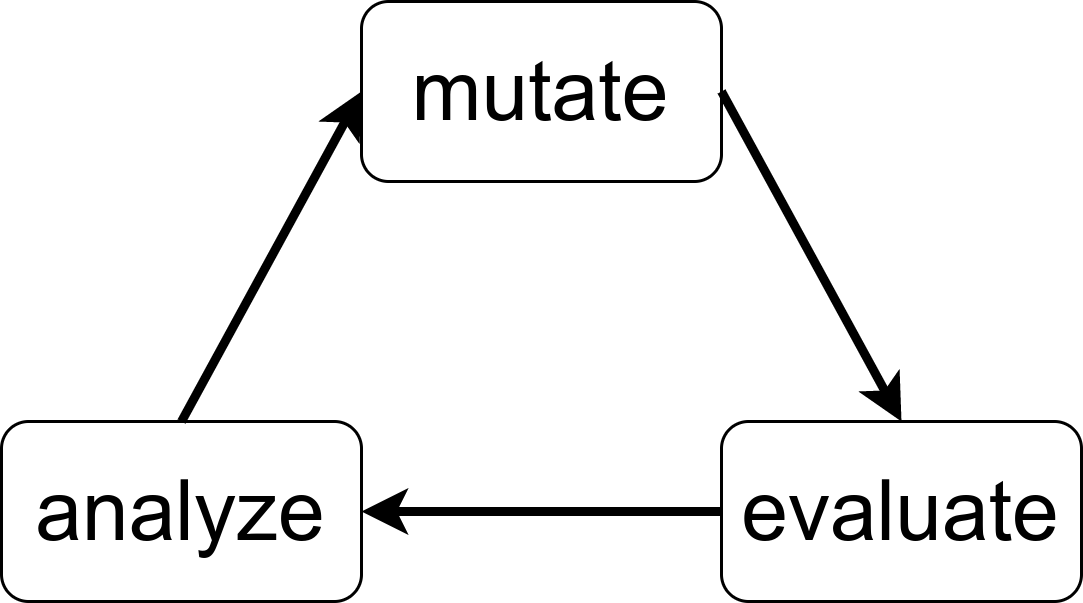
\includegraphics[width=5cm]{fuzz_loop.png}
	\end{minipage}
	\end{frame}

	\begin{frame}[t]{Подходы к генерации}
		
		\vspace{1.2cm}
		\begin{minipage}[t]{0.5\textwidth}
			\raggedright
			Эволюционный
			
			\begin{itemize}
				\item простые операции
				\item попытка взять числом
				\item необходимость выявления новых путей
			\end{itemize}
			
		\end{minipage}\begin{minipage}[t]{0.5\textwidth}
			\raggedright
			Символьное исполнение
			
			\begin{itemize}
				\item составление системы уравнений
				\item может явно перебирать пути исполнения
				\item дороговизна вычислений
			\end{itemize}
		
	\end{minipage}
			
	\end{frame}

	\begin{frame}[t]{Мутация деревьев}
		\begin{minipage}{0.5\textwidth}
			
			\vspace{1.5cm}
			
			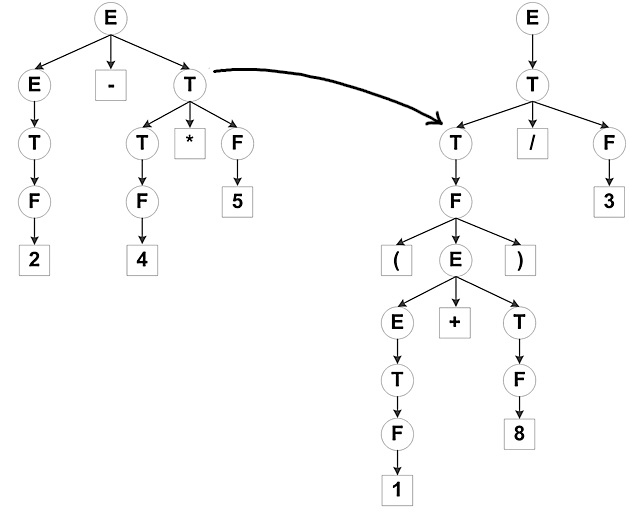
\includegraphics{tree-mutate.png}
			
		\end{minipage}\begin{minipage}{0.5\textwidth}
			
			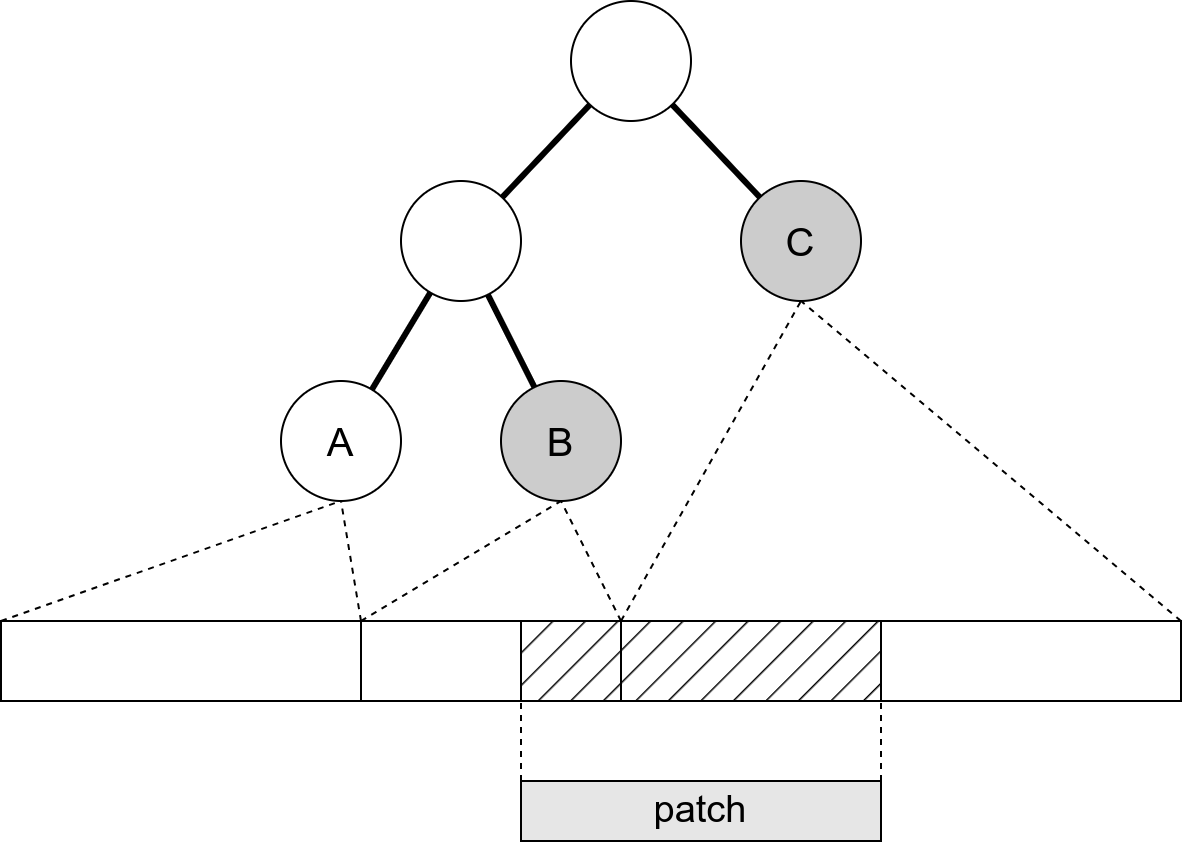
\includegraphics[width=5cm]{tree-modification.png}
		\end{minipage}
	\end{frame}

	\begin{frame}[t]{Сбор покрытия}
		\begin{minipage}{0.5\textwidth}
			
			\vspace{1.5cm}
			
			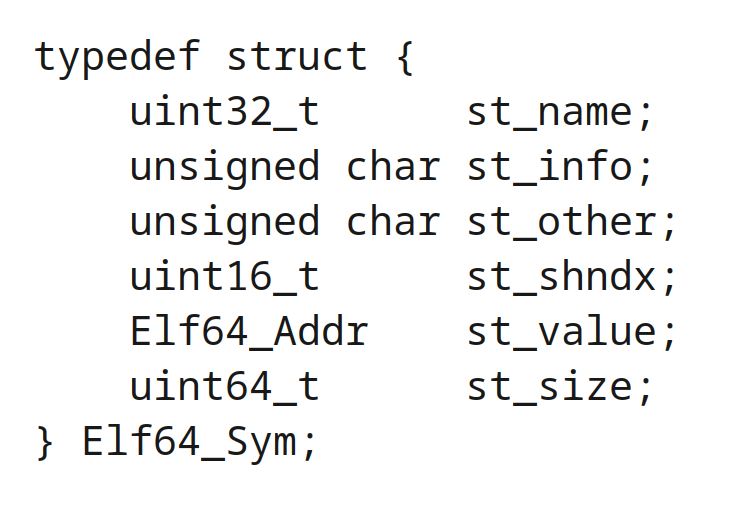
\includegraphics[width=5cm]{elf-sym.png}
			
		\end{minipage}\begin{minipage}{0.5\textwidth}
			
			\vspace{1.5cm}
			
			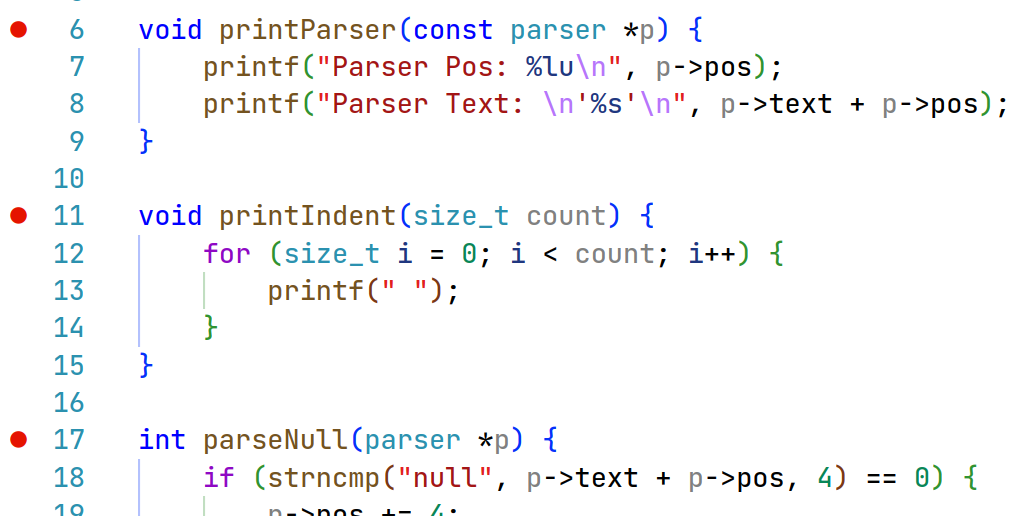
\includegraphics[width=6cm]{breakpoints.png}
		\end{minipage}
	\end{frame}

	\begin{frame}[t]{Выбор стратегий}
		\begin{minipage}{0.5\textwidth}
			
			\vspace{1.1cm}
			
			\begin{itemize}
				\item вероятность, соразмерная длине пути для образца
				
				\item применение методов для задач многоруких бандитов для выбора мутаторов
			\end{itemize}
		
			
		\end{minipage}\begin{minipage}{0.5\textwidth}
			
			\vspace{1.1cm}
			
\includegraphics[width=5cm]{bandit.png}
		\end{minipage}
	\end{frame}
	
	\begin{frame}[t]{Интерфейс}
		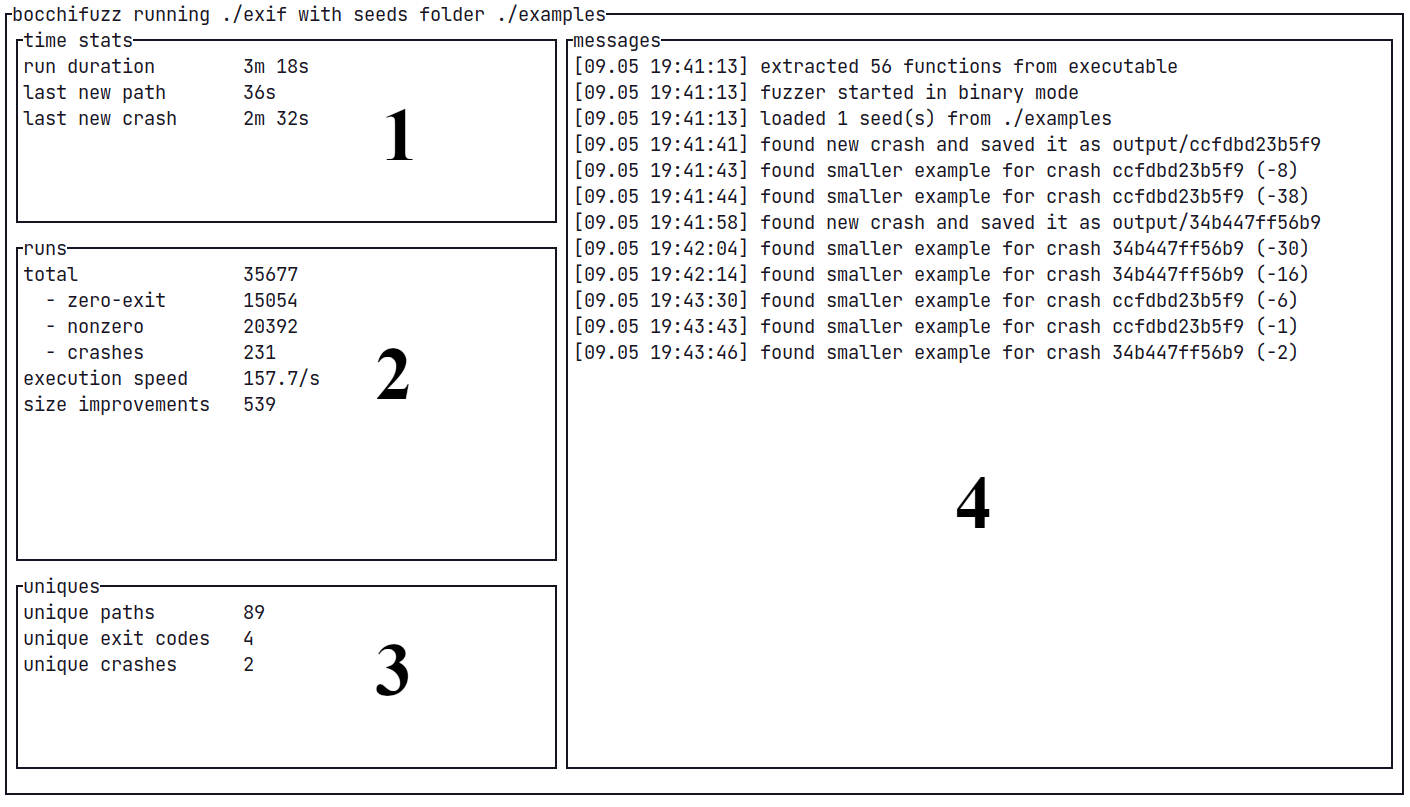
\includegraphics[width=12cm]{tui.png}
	\end{frame}

	\begin{frame}[c]
		\fontsize{26}{24}\selectfont
		\centering Спасибо за внимание!
	\end{frame}
	
\end{document}